\chapter{第二章}\label{chap2}

\section{第一节} \label{WaveAndParticles}
\subsection{第一小节} \label{EPdrift}
如图\ref{figHeidbrink2008Particles}和表\ref{tableExample}所示
\begin{figure}[htp]
	\centering
	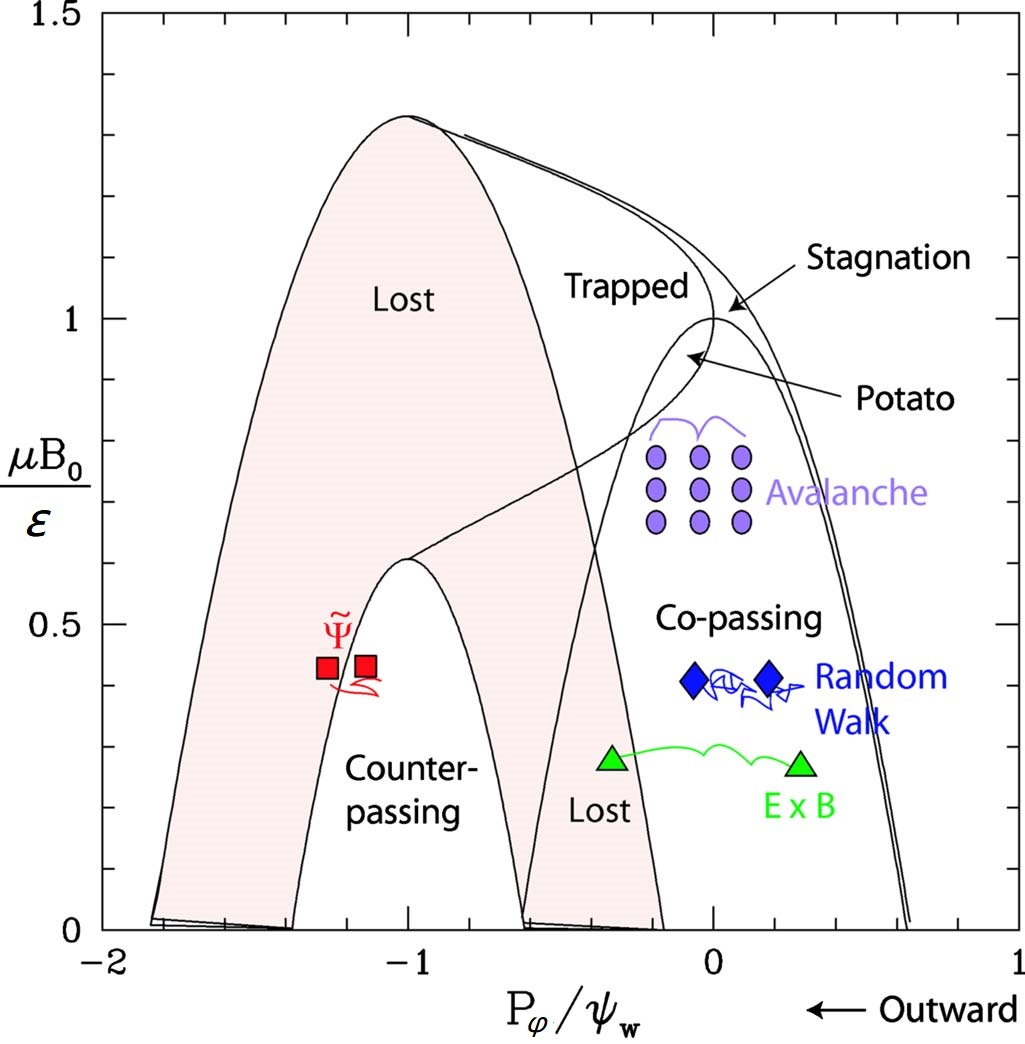
\includegraphics[width=0.45\textwidth]{./images/Heidbrink2008Particles.jpg}
	\caption{DIII-D托卡马克中中性束粒子的不同轨道类型相空间分布示意图\cite{Heidbrink2008POP}。}
	\label{figHeidbrink2008Particles}
\end{figure}


\begin{table}[htb]
    \centering
    \caption{XXXXXXXX。}
    \label{tableExample}
      \begin{tabular}{cccccc}
        \toprule
        \multicolumn{1}{m{20mm}}{\heiti\centering AAAA} & \multicolumn{1}{m{20mm}}{\heiti\centering BBBB} & \multicolumn{1}{m{20mm}}{\heiti\centering CCCC} & \multicolumn{1}{m{20mm}}{\heiti\centering DDDD} & \multicolumn{1}{m{20mm}}{\heiti\centering EEEE} & \multicolumn{1}{m{20mm}}{\heiti\centering FFFF} \\
        \midrule
        XXXX   & XXXX & XXXX & XXXX & XXXX & XXXX \\ 
		XXXX   & XXXX & XXXX & XXXX & XXXX & XXXX \\ 
        \midrule
		XXXX   & XXXX & XXXX & XXXX & XXXX & XXXX \\ 
        \bottomrule
      \end{tabular}
  \end{table}